% Apart Research AI x Epistemics Research Sprint, November 2026. Report for Track 1.
% Mirrors the section structure of Apart's official Google-Docs template (the template is not distributed as LaTeX).
% Build: pdflatex main.tex (twice). Figures: scripts/make_figures.py. Tables: scripts/make_tables.py (generated from the run's JSON).
\documentclass[10pt]{article}
\usepackage[letterpaper,margin=1in]{geometry}
\usepackage{lmodern}
\usepackage[T1]{fontenc}
\usepackage{microtype}
\usepackage{graphicx,booktabs,array,tabularx,float,enumitem,xcolor,amsmath,caption}
\usepackage[numbers,sort&compress]{natbib}
\usepackage[hidelinks]{hyperref}
\usepackage{url}
\setlength{\parindent}{1.2em}
\setlength{\parskip}{0.2em}
\setlength{\emergencystretch}{3em}
\setlist{nosep,leftmargin=1.6em}
\captionsetup{font=small,labelfont=bf,skip=4pt}
\renewcommand{\paragraph}[1]{\par\vspace{0.3em}\noindent\textit{#1}\ }
\newcommand{\code}[1]{\texttt{#1}}

\title{\vspace{-1.2em}A Linear Answerability Signal That the Model Does Not Act On:\\Probes, Verbal Confidence and an Abstain Option in Phi-3.5-mini\thanks{Research conducted at the AI x Epistemics Research Sprint, November 2026.}}
\author{Mackenzie O'Brien\\ Mac Labs AI\\[2pt] \small With Apart Research}
\date{}

\begin{document}
\maketitle
\vspace{-2.2em}

\begin{abstract}
\noindent
We ask whether Phi-3.5-mini-instruct (3.8B parameters, 8-bit) carries a linearly readable signal for whether a question is answerable, and whether its stated confidence or abstention behaviour reflects that signal. On SQuAD 2.0 (1,200 balanced questions, passage-disjoint 60/20/20 splits, test n=240), a logistic probe on the last prompt token reaches an area under the ROC curve (AUROC) of 0.906 (95\% confidence interval, CI, 0.867--0.948) at layer 18, chosen on validation data. Verbalized confidence reaches 0.621, token-level and sampling signals 0.665--0.688, question length 0.569, and probes trained on shuffled labels 0.492. The behavioural counterpart is weak: the model abstains on 5\% of unanswerable test items, and an explicit UNANSWERABLE option raises this to 15\% with precision 1.0 (18 of 18). On 46.7\% of all test items the probe says unanswerable while the model commits with confidence at least 0.8, and those items are wrong 82.1\% of the time, against 52.5\% overall. SelfAware gives a probe AUROC of 0.993, but a source-only feature reaches 1.000, so we report it as a confound; transfer between the two datasets is weak (0.58 and 0.67). We claim a linear signal that predicts answerability within SQuAD under length and shuffle controls, from one model, one run and one prompt. We do not claim that the model knows it does not know.
\end{abstract}

%====================================================================
\section{Introduction}
%====================================================================
A model that answers every question in the same confident tone leaves its reader unable to tell which answers to trust, and the problem is sharpest when the evidence needed for an answer is missing. We study a narrow version of it. When Phi-3.5-mini-instruct \citep{abdin2024phi3} reads a passage and a question that the passage cannot answer, does its hidden state carry a linearly readable trace of that fact, and does anything the model says or does reflect the trace? This is an evaluation question for Track~1 of the sprint, because it asks whether a model's expressed confidence can be checked against an internal signal and against ground truth about answerability.

We use two benchmarks with different meanings of ``unanswerable''. SQuAD 2.0 contains questions whose answer is absent from a given passage, written by crowdworkers to resemble answerable ones \citep{rajpurkar2018squad2}. SelfAware contains questions that cannot be answered at all, for example because experts disagree, mixed with answerable questions drawn from other datasets \citep{yin2023selfaware}. We planned to treat both as probe targets. An audit changed the plan: every unanswerable SelfAware question carries the source label \code{SelfAware}, so a classifier that sees only the source scores AUROC 1.000, and the probe's 0.993 on that set says little about answerability. We therefore report SQuAD 2.0 as the primary result and SelfAware as a documented confound.

Earlier work has already found answerability information in the hidden states of language models \citep{slobodkin2023curious,lavi2026directions,wagner2026twoaxes}, so we do not present the existence of such a signal as new. Our contribution is a controlled, fully specified measurement on a small open model, with every selection step made on validation data, and a careful account of what the behavioural comparisons do and do not show. Our main contributions are:
\begin{enumerate}
\item A layer-wise probe study on SQuAD 2.0 (test n=240): a logistic probe reaches AUROC 0.906 [0.867, 0.948] at a validation-chosen layer, well above verbal confidence (0.621), token log-probability (0.667), token entropy (0.688), a question-length baseline (0.569), and a shuffled-label null (mean 0.492, maximum 0.568).
\item An audit of source confounds: SelfAware and pooled probe scores (0.993, 0.959) are not evidence of answerability coding, since source alone gives 1.000 on SelfAware and a question-only bag-of-words classifier gives 0.923; transfer between SQuAD and SelfAware is weak (0.580 and 0.671 at the source's own best layer).
\item Behavioural gap measures with explicit definitions: a recognition--action gap of 0.296, a gap rate of 46.7\% of all test items (error rate 0.821 against 0.525 overall), and an explicit abstain option that flags 15\% of unanswerable items, all correctly. We state why each of these is partly a consequence of prompt design and of near-saturated verbal confidence.
\end{enumerate}

%====================================================================
\section{Related Work}
%====================================================================
\paragraph{Answerability and self-knowledge.}
SQuAD 2.0 added unanswerable questions to extractive reading comprehension so that systems must decide when to abstain \citep{rajpurkar2018squad2}. SelfAware evaluates whether language models can identify questions that have no definite answer and reports a gap between models and humans \citep{yin2023selfaware}. Kalai et al.\ argue that binary-graded benchmarks reward guessing over admitting uncertainty, which motivates measuring abstention directly \citep{kalai2025hallucinate}.

\paragraph{Expressed uncertainty.}
Models can be asked to judge their own answers \citep{kadavath2022know}, to state confidence in words \citep{lin2022words,xiong2024express}, or to be checked for agreement across samples \citep{manakul2023selfcheck,kuhn2023semantic}. We use a verbalized 0--100 confidence elicited in a follow-up turn, token log-probability and entropy of the answer, and a simple agreement rate over five samples; we do not implement semantic clustering or the P(True) and P(IK) protocols.

\paragraph{Probing internal states.}
Linear probes on hidden states can predict whether a statement is true \citep{azaria2023internal,burns2023ccs,marks2024geometry}, and control tasks help separate what a probe reads from what it can learn by itself \citep{hewitt2019control,belinkov2022probing}. We use a logistic probe and the difference-of-means (mass-mean) probe of \citet{marks2024geometry} as a robustness check, and we follow the control-task spirit of \citet{hewitt2019control} with shuffled-label and surface-feature baselines.

\paragraph{Answerability in hidden states.}
Slobodkin et al.\ report that models appear to encode whether a query is answerable even when they hallucinate an answer \citep{slobodkin2023curious}. Lavi et al.\ find a linear unanswerability direction in extractive QA, test its transfer to SelfAware, and show that adding or ablating it changes abstention \citep{lavi2026directions}. Wagner separates answer correctness from question answerability and finds that a hidden-state probe tracks the second while answer confidence tracks the first \citep{wagner2026twoaxes}. Two further papers study mechanism: Nguyen et al.\ localise a commit--abstain circuit across ten models \citep{nguyen2026cac}, and Ferrando et al.\ find entity-recognition directions that causally affect refusal \citep{ferrando2025entity}. Relative to this work we study one small model and make no causal intervention, but we add a SelfAware source-confound audit, validation-only selection throughout, and explicit definitions of the gap measures. We do not claim that the signal is new or causal.

%====================================================================
\section{Methods}
%====================================================================
\subsection{Model, prompts and generation}
We run \code{microsoft/Phi-3.5-mini-instruct} (3.8B parameters, 32 transformer layers, hidden size 3072) in 8-bit quantization on a single GPU with 8~GB of memory, batch size one, because the bf16 weights do not fit. Quantization changes hidden states slightly relative to bf16, and we did not measure the effect. Answers are greedy with at most 32 new tokens; prompts are truncated from the left to 1,024 tokens (we did not log how many prompts were affected). The system message is ``You are a careful assistant. Answer concisely.'' For SQuAD the user message asks the model to answer using the passage with a few words, followed by the passage and question; for SelfAware it contains the question only. Appendix~\ref{app:prompts} gives the exact text.

We make three model calls per item. The plain prompt, which offers no abstention option, yields the answer, its token log-probabilities and entropies, and the hidden states we probe. A second turn appended to the same conversation asks ``How confident are you that your answer is correct?'' on a 0--100 scale, and we parse the first number and divide by 100. A third call repeats the plain prompt with one added sentence, ``If the question cannot be answered, reply exactly UNANSWERABLE.'', which we call the explicit abstain option. For a hash-selected 25\% of items (807 of 3,200, including 51 of the 240 SQuAD test items) we also draw five samples at temperature 0.7, and the consistency signal is the share of samples whose normalised string equals the normalised greedy answer.

\subsection{Data and splits}
SQuAD 2.0 uses the official development set (11,873 questions, 5,945 unanswerable). We take 600 answerable and 600 unanswerable questions in SHA-256 hash order and split by passage, stratified by class, into 720/240/240 train/validation/test items, so no passage appears in two splits. SelfAware (file with 2,338 answerable and 1,031 unanswerable questions) is subsampled to 1,000 per class and split by question into 1,200/400/400. The pooled set has 3,200 items (1,920/640/640). SQuAD test has 120 answerable and 120 unanswerable items. Seeds, subsampling and splits are deterministic (seed 13); the single run reported here is \code{20261114T041458Z-full--apart}.

\subsection{Probes}
For each of the 33 residual-stream positions (embedding output plus 32 layers) we take the hidden state at the final token of the chat-formatted plain prompt, the position from which the first answer token is generated. Features are standardised with training-set mean and standard deviation. The primary probe is an L2-regularised logistic regression (scikit-learn defaults, $C=1$, up to 1,000 iterations) with label answerable $=1$, trained on the training split only. We also fit a mass-mean probe (difference of class means with a midpoint bias) as a robustness check. The reported layer is the one with the highest validation AUROC. The probe score is the logit, and ``the probe says unanswerable'' means a score below the threshold that maximises Youden's J (true-positive rate minus false-positive rate) on the validation split.

\subsection{Baselines and controls}
We score four expressed signals for answerability with the same AUROC: verbalized confidence, mean token log-probability of the answer, negative mean token entropy, and consistency. The explicit abstain option enters as one hard decision. Three controls guard the probe against artifacts. In the shuffled-label control we permute the training labels and repeat the whole layer-wise protocol, including layer selection on validation, 20 times. The length baseline is a logistic regression on question word count, question characters or prompt characters. A post hoc lexical check (Appendix~\ref{app:lexical}) fits TF-IDF and question--passage word-overlap features on the same splits, and Appendix~\ref{app:posthoc} lists which numbers come from the run's analysis files and which we computed afterwards.

\subsection{Scoring and metrics}\label{sec:metrics}
SQuAD answers count as correct on exact match or token-F1 $\geq 0.5$ against any gold answer; on an unanswerable item an answer is correct only if it abstains. SelfAware answers are scored by normalised string containment, which misses paraphrases. Abstention is detected by a rule list (for example ``UNANSWERABLE'', ``cannot be answered'', ``I don't know''); no model or human judge audited it, and a reply such as a confident but unsupported negation is counted as an answer.

All AUROCs are rank-based with average ranks for ties. Intervals are 95\% percentile bootstrap intervals over test items (300 resamples, seed 13), which resample items independently and so ignore clustering by passage. We call the \emph{gap rate} the share of all test items for which (i) the probe says unanswerable, (ii) the model did not abstain under the plain prompt, and (iii) verbalized confidence is at least 0.8; the \emph{error rate in the gap} is the share of those items that the model answered incorrectly, counting any answer to an unanswerable item as incorrect. The \emph{recognition} score is the balanced accuracy of the probe at its validation threshold. The \emph{action} score is the balanced accuracy of the model's own behaviour, the mean of the share of answerable items it answers and the share of unanswerable items it abstains on, and the \emph{recognition--action gap} is recognition minus action. Abstention precision and recall are computed for the unanswerable class.

\subsection{Selection protocol}
Table~\ref{tab:protocol} lists what was chosen on which split. The only quantities selected on test data are the ``maximum over layers'' transfer figures, which we label as optimistic and do not use as headline results. We ran one seed on one split, so no variance across seeds or splits is available.

\begin{table}[t]
\centering\small
\caption{What was chosen on which split.}
\label{tab:protocol}
\begin{tabular}{@{}p{0.43\linewidth}p{0.25\linewidth}p{0.25\linewidth}@{}}
\toprule
Choice & Made on & Reported on \\
\midrule
Probe layer (L18 for SQuAD) & validation AUROC & test \\
Probe and verbal-confidence thresholds & validation Youden's J & test \\
Probe regularisation ($C=1$), confidence cut (0.8) & fixed in the config before the run & test \\
Transfer layer, ``reported'' column & source dataset's validation & target test \\
Transfer layer, ``maximum over layers'' & target test (optimistic) & target test \\
Splits, subsampling, bootstrap and shuffle seeds & fixed (seed 13) & -- \\
\bottomrule
\end{tabular}
\end{table}

%====================================================================
\section{Results}
%====================================================================
\paragraph{A linear signal separates answerable from unanswerable SQuAD questions at middle layers.}
The logistic probe reaches test AUROC 0.906 (95\% CI 0.867--0.948, n=240) at layer 18, the layer with the best validation AUROC (0.918). Figure~\ref{fig:layers} shows the layer profile: test AUROC stays at or below 0.668 through layer 11, rises to 0.865 at layer 15, peaks at 0.918 at layer 17, and declines to 0.832 at layer 32; layer 0 scores exactly 0.500, as it must when every item ends in the same token. The layer with the highest test AUROC (17) is one layer from the validation choice and 0.012 above the reported value, so the reported number is not inflated by selecting on test data. The mass-mean probe selects the same layer and reaches 0.927 on test (validation 0.912), so the result does not hinge on the logistic fit. At the validation threshold the probe has balanced accuracy 0.821. Table~\ref{tab:layers} gives all 33 layers.

\begin{figure}[t]
\centering
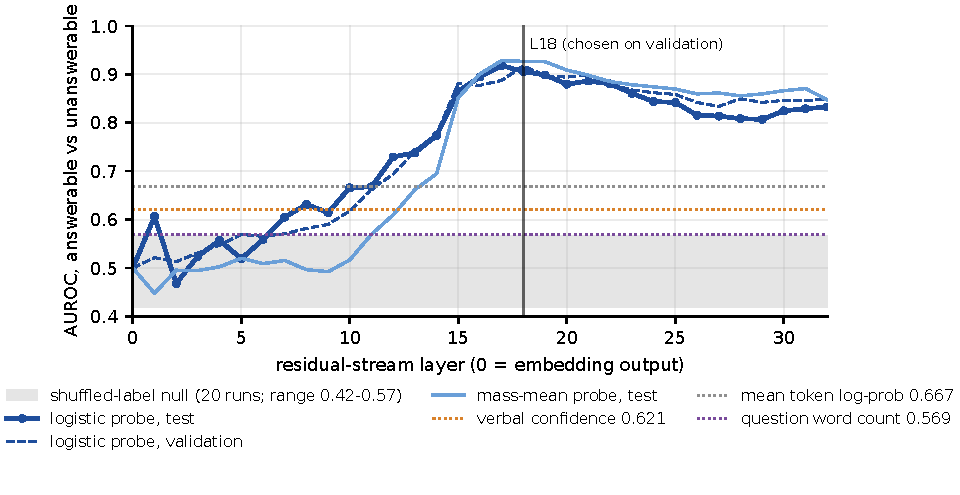
\includegraphics[width=0.8\linewidth]{figures/fig_layers.pdf}
\caption{Probe AUROC by layer on SQuAD 2.0 (n=240 per split). The shaded band is the range of 20 shuffled-label runs under the same selection protocol. Dotted lines are single-signal baselines on the same test items. The vertical line marks the layer chosen on validation.}
\label{fig:layers}
\end{figure}

\paragraph{Controls bound what a trivial feature can explain.}
Probes trained on shuffled labels reach a mean test AUROC of 0.492 (SD 0.039, range 0.418--0.568, 20 runs, none above 0.8), so layer selection on 240 validation items does not by itself produce a high score. Question length is a weak predictor: logistic AUROC 0.569 on word count, 0.558 on characters, 0.497 on prompt characters and 0.557 on all three, with answerable and unanswerable questions averaging 10.2 and 9.8 words. A post hoc lexical check gives 0.598 for TF-IDF of the question, 0.600 for question--passage word overlap and 0.635 for both (Appendix~\ref{app:lexical}). These baselines do not exclude other surface cues, such as artifacts of how crowdworkers wrote the unanswerable questions, and we did not test for them.

\begin{figure}[t]
\centering
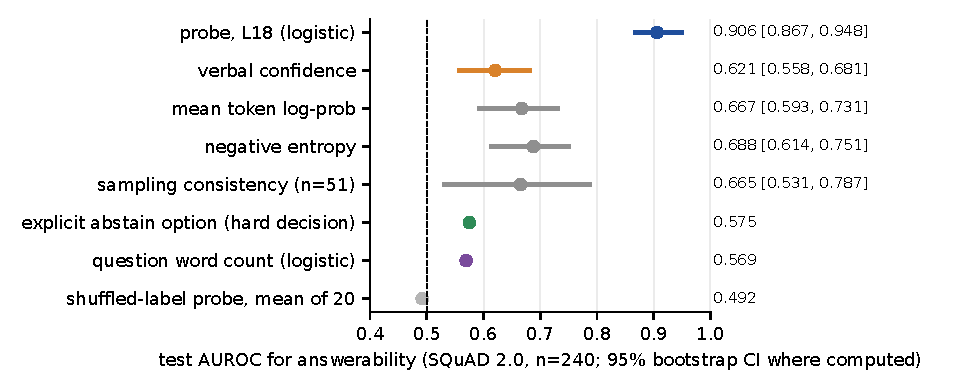
\includegraphics[width=0.85\linewidth]{figures/fig_signals.pdf}
\caption{Test AUROC for answerability on SQuAD 2.0 for the probe, expressed signals and controls. Bars are 95\% bootstrap intervals where the run computed them. Consistency exists for 51 of the 240 test items only. The abstain option is one hard decision, so its AUROC equals its balanced accuracy.}
\label{fig:signals}
\end{figure}

\paragraph{Expressed signals track answer correctness better than answerability.}
Verbalized confidence scores 0.621 [0.558, 0.681], mean token log-probability 0.667 [0.593, 0.731], negative entropy 0.688 [0.614, 0.751], and sampling consistency 0.665 [0.531, 0.787] on only 51 items (Figure~\ref{fig:signals}, Table~\ref{tab:signals}); the probe's interval lies above all of them, though we ran no paired test. The ordering reverses for answer correctness among answerable items: AUROC is 0.799 for verbal confidence, 0.869 for log-probability and 0.894 for entropy, against 0.660 for the probe, with only 12 incorrectly answered items among the 120. This pattern matches the two-axes account of \citet{wagner2026twoaxes}: expressed confidence follows whether an answer is right, while the probe follows the label it was trained on. Verbalized confidence is also saturated. It averages 0.926 on the test split, where 47.5\% of items receive appropriate behaviour (a correct answer, or an abstention on an unanswerable item), giving an expected calibration error of 0.484 with ten equal-width bins. The distribution is bimodal, with 227 items near 0.98 (appropriate 0.485) and 13 items near 0 (appropriate 0.308).

\begin{table}[t]
\centering\small
\caption{Answerability signals on the SQuAD~2.0 test split (n=240; 120 answerable, 120 unanswerable). AUROC columns use the raw signal; the 95\% interval is a percentile bootstrap over test items (300 resamples). The right-hand block thresholds each signal at the cut that maximises Youden's J on the validation split, then scores flagging an item as unanswerable (precision, recall and F1 are for the unanswerable class; coverage is the share of items still answered). The explicit abstain option is a single hard decision, so its AUROC equals its balanced accuracy and it has no threshold. Sampling consistency exists for only 51 test items (23 answerable), so its AUROC is not comparable with the others and its thresholded columns are omitted (items without a score would be silently counted as answered).}
\label{tab:signals}
\resizebox{\linewidth}{!}{\begin{tabular}{@{}lccccccc@{}}
\toprule
Signal & AUROC (answerability) & 95\% CI & AUROC (correctness) & Coverage & Prec. & Recall & F1 \\
\midrule
Linear probe, L18 & 0.906 & [0.867, 0.948] & 0.660 & 0.471 & 0.803 & 0.850 & 0.826 \\
Verbal confidence & 0.621 & [0.558, 0.681] & 0.799 & 0.879 & 0.828 & 0.200 & 0.322 \\
Mean token log-prob & 0.667 & [0.593, 0.731] & 0.869 & 0.583 & 0.660 & 0.550 & 0.600 \\
Negative entropy & 0.688 & [0.614, 0.751] & 0.894 & 0.571 & 0.670 & 0.575 & 0.619 \\
Sampling consistency (n=51) & 0.665 & [0.531, 0.787] & 0.977$^{\dagger}$ & -- & -- & -- & -- \\
Explicit abstain option & 0.575 & -- & -- & 0.925 & 1.000 & 0.150 & 0.261 \\
Question word count (logistic) & 0.569 & -- & -- & -- & -- & -- & -- \\
Shuffled-label probe (mean of 20) & 0.492 & -- & -- & -- & -- & -- & -- \\
\bottomrule
\end{tabular}}
\par\vspace{2pt}{\footnotesize $^\dagger$ Computed on the 23 answerable test items that have a consistency score, only one of which was answered wrongly, so this value rests on 22 pairs and is not reliable. The correctness AUROC of the other signals uses the 120 answerable test items, 12 of which were answered wrongly.}
\end{table}


\paragraph{The probe and the model's behaviour disagree on most unanswerable items.}
Under the plain prompt the model answers 90.0\% of answerable test questions correctly and abstains on 6 of 120 unanswerable ones (5.0\%), and on none of the answerable ones. The recognition score is 0.821 and the action score 0.525, a recognition--action gap of 0.296 (post hoc 95\% CI 0.240--0.344). The probe flags 127 of the 240 test items as unanswerable (102 truly so, 25 answerable). Of these, 112 (88.2\%) are items the model answered without abstaining at stated confidence of at least 0.8, which is 46.7\% of all test items (post hoc CI 41.0--52.9\%; Figure~\ref{fig:gap}). Of the 112, 87 are unanswerable and 25 answerable, and 92 are answered wrongly, an error rate of 0.821 (post hoc CI 0.747--0.888). The comparison rates are 0.525 over all 240 items and 0.266 over the 128 items outside the gap. Among the 120 unanswerable items, 87 (72.5\%) fall in the gap.

\begin{figure}[t]
\centering
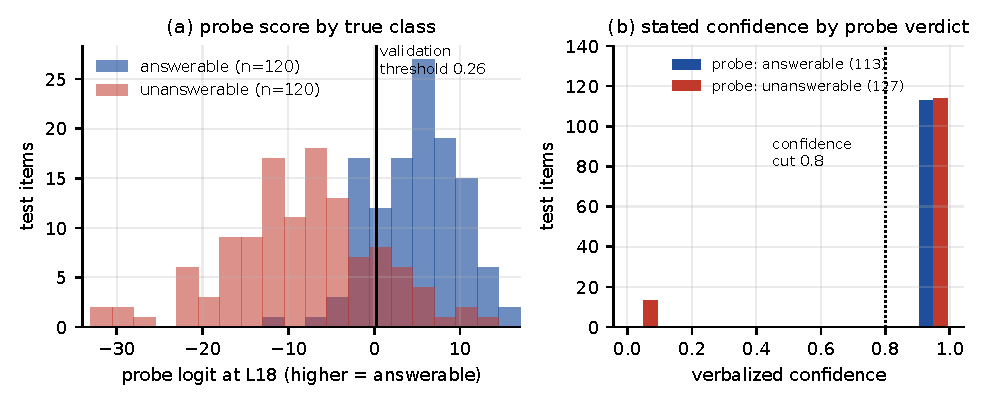
\includegraphics[width=0.92\linewidth]{figures/fig_gap.pdf}
\caption{(a) Probe logit at layer 18 by true class on the SQuAD test split; the line is the threshold chosen on validation. (b) Verbalized confidence by probe verdict. All 113 items the probe calls answerable have confidence above 0.9; of the 127 it calls unanswerable, 114 do too and 13 sit near zero.}
\label{fig:gap}
\end{figure}

Two features of this measurement limit its reading. First, the confidence condition barely filters: 225 of the 240 items are answered at confidence at least 0.8 (error rate 0.520), so the gap rate is close to the share of items the probe flags and the model does not decline. Second, the plain prompt offers no way to decline, so a low action score is expected of any model that follows the instruction to answer; with the explicit option the action score is 0.575 and the recognition--action gap 0.246 (post hoc CI 0.189--0.292). The gap therefore measures that a supervised probe, trained on 720 labelled items, recovers a distinction the model does not act on under these two prompts. It does not show the model ``withholds'' anything.

\begin{table}[t]
\centering\small
\caption{Thresholded flagging of unanswerable SQuAD test items (n=240; 120 unanswerable). Probe and verbal-confidence thresholds were fitted on validation labels; the abstain option used no labels. ``False abstention'' is the share of correctly answered answerable items that the rule would have refused.}
\label{tab:flagging}
\begin{tabular}{@{}lccccc@{}}
\toprule
Rule & Recall & Precision & F1 & Coverage & False abstention \\
\midrule
Probe, L18 & 0.850 & 0.803 & 0.826 & 0.471 & 0.185 \\
Verbal confidence $<0.95$ & 0.200 & 0.828 & 0.322 & 0.879 & 0.037 \\
Explicit abstain option & 0.150 & 1.000 & 0.261 & 0.925 & 0.000 \\
\bottomrule
\end{tabular}
\end{table}

\paragraph{An explicit abstain option adds little recall.}
With the sentence ``reply exactly UNANSWERABLE'' appended, the model abstains on 18 of 120 unanswerable test items and on none of the answerable ones, so precision is 1.0 (18 of 18) and recall 0.150 (post hoc CI 0.091--0.208); F1 is 0.261 and the balanced accuracy, which is also its AUROC, is 0.575 (Table~\ref{tab:flagging}; Appendix Figure~\ref{fig:ops}). The option is conservative rather than inaccurate: it never refuses an answerable question, but it leaves 102 of 120 unanswerable questions answered, and the share of items with appropriate behaviour moves only from 0.475 to 0.521. Table~\ref{tab:flagging} shows that the probe at its validation threshold has the highest F1 and verbal confidence the next; however, those two thresholds used validation labels and the option did not, so the comparison favours them. We tried one wording of the option, and a different prompt might raise recall. For the probe, flagging at the validation threshold keeps 47.1\% coverage and raises accuracy among answered items from 0.450 to 0.779, at the price of refusing 18.5\% of correct answers.



\paragraph{SelfAware and pooled probe scores are source-confounded, and transfer is weak.}
On SelfAware the probe reaches 0.993 [0.985, 0.998] at layer 15 (test n=400), yet a logistic classifier on the source label alone reaches 1.000, because all 1,000 unanswerable items have source \code{SelfAware} and none of the 1,000 answerable items does (Table~\ref{tab:crosstab}). A TF-IDF classifier on the question text reaches 0.923 in a post hoc check, which indicates that question style alone separates the classes. The pooled probe scores 0.959 [0.944, 0.972] at layer 18 (n=640), where a source-only feature gives 0.930; this is not 1.000 because the SQuAD half shares one source across both classes. We treat both as confounds and not as evidence (Table~\ref{tab:datasets}).

A SelfAware-trained probe scored on the SQuAD test split gives AUROC 0.580 at its validation-chosen layer (15); the best of the 33 layers on SQuAD test is 0.788 at layer 19, which was picked on the target test set and is an optimistic upper bound. A SQuAD-trained probe scored on the SelfAware test split gives 0.671 at layer 18, with a test-picked maximum of 0.728 at layer 10 (Table~\ref{tab:transfer}, Appendix Figure~\ref{fig:transfer}). Transfer is weak in both directions, which is what a source or style probe would produce and is not what a probe of a general answerability variable would be expected to produce. The SQuAD$\to$SelfAware figure is above chance but cannot separate shared answerability structure from other differences between the datasets.

\paragraph{The development run gave a lower figure, which we attribute to sample size.}
A 400-item development run of the same pipeline (100 questions per class per dataset, no consistency or abstain-option pass) gave a SQuAD probe AUROC of 0.821 at layer 19, against 0.906 at layer 18 in the full run. The development test split has 41 SQuAD items, and its bootstrap interval (100 resamples) is 0.664--0.939, which contains the full-run value. At layer 19 the full run gives a test AUROC of 0.899. The development items come from the same hash ordering as the full pool and so are a subset of it, but the split assignment differs, which means the development run is not an independent replication. We did not test this explanation beyond the interval overlap, and we regard the difference as most likely sampling noise in a small test set, not as a measured effect.

%====================================================================
\section{Discussion and Limitations}
%====================================================================
\paragraph{Discussion.}
Within SQuAD 2.0, a linear readout from middle layers separates answerable from unanswerable questions far better than question length, lexical overlap, shuffled labels, or any signal the model expresses, and the pattern is stable across a logistic and a difference-of-means probe. A natural reading is that, by layers 15 to 19, the prompt representation encodes whether the passage supports an answer, since a model that must produce a span answer needs some such computation. That reading is a hypothesis; our experiments do not intervene on the representation. The behavioural side is consistent with the idea that this information is not routed into the model's refusal behaviour or confidence under the prompts we used, but we cannot separate a model limitation from an elicitation limitation, since our confidence question asks about the correctness of an answer, which has no meaning for an unanswerable item, and our abstain option is a single wording.

For practice, the probe suggests a cheap gate: at the validation threshold it flags 85\% of unanswerable items at 80\% precision, but it also refuses 18.5\% of correct answers and requires white-box access and labelled training data. The SelfAware result is a methodological warning more than a finding. A probe can reach 0.993 AUROC on a benchmark where a one-feature source classifier reaches 1.000, so probe results on benchmarks assembled from heterogeneous sources need a source audit before they are read as evidence about what a model represents.

\paragraph{What this does not show.}
The probe is a supervised linear predictor of a dataset label, so a high AUROC shows linear decodability and not that the model knows it does not know or uses the signal. Nothing here is causal, because we made no interventions, and nothing shows that the signal is the same direction across layers or datasets. The comparison with expressed uncertainty also stops short of a general claim that the probe beats it: our verbal-confidence question concerns answer correctness, we elicited it once with one prompt, and we ran no prompted answerability question, P(True) or P(IK) baseline. Generality is limited to one 3.8B model in 8-bit, two English benchmarks, one prompt format and one seed. Finally, the recognition--action and gap numbers depend on the validation-chosen threshold, on the 0.8 confidence cut and on the plain prompt's lack of an abstain option.

\paragraph{Limitations.}
Statistical power is limited. The SQuAD test split has 240 items, 120 per class, only 12 of the answerable ones were answered wrongly, and the consistency signal covers 51 items. All comparisons reuse the same test items, with no multiple-comparison correction and no paired tests, and the bootstrap intervals ignore passage clustering. No judge audited the rule-based abstention detector, so soft refusals phrased in unexpected ways, or hallucinated denials, may be misclassified, and the string-containment scoring of SelfAware answers understates accuracy. The probe sees only the plain prompt while the abstain-option pass uses a different prompt, so the option and the probe are not evaluated on identical inputs. We did not log how many prompts were truncated at 1,024 tokens, and 8-bit quantization may shift hidden states. SQuAD's unanswerable questions were written adversarially, so surface artifacts beyond those we tested may exist. Last, the abstain-option analysis code was added to the repository after the run, and we recomputed its numbers from the run's saved responses (Appendix~\ref{app:posthoc}).

\paragraph{Future work.}
The most informative next steps are an interventional test (adding or ablating the probe direction and measuring abstention, in the manner of \citet{lavi2026directions}), a prompted answerability question and P(True) baseline, several abstain-option wordings, multiple seeds and splits, a second model, and an unconfounded inherent-unanswerability dataset in which source does not alias the label.

%====================================================================
\section{Conclusion}
%====================================================================
On SQuAD 2.0, a layer-18 linear probe in Phi-3.5-mini-instruct predicts answerability with AUROC 0.906 [0.867, 0.948] under length, shuffle and lexical controls. The model's verbal confidence (0.621) and an explicit abstain option (0.575, recall 0.15) do much worse. The SelfAware and pooled scores are source artifacts and cross-dataset transfer is weak, so the claim stays within SQuAD: a linear signal that predicts answerability for one model, one run and one prompt.

\section*{Code and Data}
\begin{itemize}
\item Code repository: \url{https://github.com/mso-docs/Apart-Epistemics}
\item Data: SQuAD 2.0 \citep{rajpurkar2018squad2} and SelfAware \citep{yin2023selfaware} are public (CC BY-SA 4.0): \url{https://rajpurkar.github.io/SQuAD-explorer/} and \url{https://github.com/yinzhangyue/SelfAware}. The repository's source list records the download URL, size and SHA-256 of each file. Our processed items and per-item model outputs are in the dataset \url{https://huggingface.co/datasets/mackenzietechdocs/apart-epistemics-phi35-abstention}.
\item Run outputs: run \code{20261114T041458Z-full--apart} (analysis files \code{metrics.json}, \code{sanity.json}, \code{curves.json}, \code{probe\_scores.jsonl}, \code{abstain\_option.json}), released in the dataset above together with the \code{items.jsonl} file and the Evalboard interpretability artifacts.
\item New work versus prior work: all code, experiments and writing for this report were done during the sprint (November 13--15, 2026), and no code or results predate it. We build on third-party software (PyTorch, Transformers, bitsandbytes, scikit-learn), public datasets and the public model weights, all cited or named above.
\end{itemize}

\section*{Author Contributions}
Mackenzie O'Brien is the sole author and did all of the work: she designed the study, wrote the code, ran the experiments, analysed the results and wrote this report.

%====================================================================
\begin{thebibliography}{99}\small
\setlength{\itemsep}{1pt}
\bibitem[Abdin et~al.(2024)]{abdin2024phi3} M.~Abdin et~al. Phi-3 technical report: A highly capable language model locally on your phone. arXiv:2404.14219, 2024.
\bibitem[Azaria and Mitchell(2023)]{azaria2023internal} A.~Azaria and T.~Mitchell. The internal state of an LLM knows when it's lying. In \emph{Findings of EMNLP 2023}, pages 967--976, 2023. arXiv:2304.13734.
\bibitem[Belinkov(2022)]{belinkov2022probing} Y.~Belinkov. Probing classifiers: Promises, shortcomings, and advances. \emph{Computational Linguistics}, 2022. arXiv:2102.12452.
\bibitem[Burns et~al.(2023)]{burns2023ccs} C.~Burns, H.~Ye, D.~Klein, and J.~Steinhardt. Discovering latent knowledge in language models without supervision. In \emph{ICLR 2023}. arXiv:2212.03827.
\bibitem[Ferrando et~al.(2025)]{ferrando2025entity} J.~Ferrando, O.~Obeso, S.~Rajamanoharan, and N.~Nanda. Do I know this entity? Knowledge awareness and hallucinations in language models. In \emph{ICLR 2025}. arXiv:2411.14257.
\bibitem[Hewitt and Liang(2019)]{hewitt2019control} J.~Hewitt and P.~Liang. Designing and interpreting probes with control tasks. In \emph{EMNLP 2019}. arXiv:1909.03368.
\bibitem[Kadavath et~al.(2022)]{kadavath2022know} S.~Kadavath et~al. Language models (mostly) know what they know. arXiv:2207.05221, 2022.
\bibitem[Kalai et~al.(2025)]{kalai2025hallucinate} A.~T. Kalai, O.~Nachum, S.~S. Vempala, and E.~Zhang. Why language models hallucinate. arXiv:2509.04664, 2025.
\bibitem[Kuhn et~al.(2023)]{kuhn2023semantic} L.~Kuhn, Y.~Gal, and S.~Farquhar. Semantic uncertainty: Linguistic invariances for uncertainty estimation in natural language generation. In \emph{ICLR 2023}. arXiv:2302.09664.
\bibitem[Lavi et~al.(2026)]{lavi2026directions} M.~J. Lavi, T.~Milo, and M.~Geva. Detecting (un)answerability in large language models with linear directions. In \emph{Proceedings of EACL 2026 (Long Papers)}, pages 682--699, 2026. arXiv:2509.22449.
\bibitem[Lin et~al.(2022)]{lin2022words} S.~Lin, J.~Hilton, and O.~Evans. Teaching models to express their uncertainty in words. arXiv:2205.14334, 2022.
\bibitem[Manakul et~al.(2023)]{manakul2023selfcheck} P.~Manakul, A.~Liusie, and M.~J.~F. Gales. SelfCheckGPT: Zero-resource black-box hallucination detection for generative large language models. In \emph{EMNLP 2023}. arXiv:2303.08896.
\bibitem[Marks and Tegmark(2024)]{marks2024geometry} S.~Marks and M.~Tegmark. The geometry of truth: Emergent linear structure in large language model representations of true/false datasets. In \emph{COLM 2024}. arXiv:2310.06824.
\bibitem[Nguyen et~al.(2026)]{nguyen2026cac} V.~Nguyen et~al. The commit-abstain circuit: Why language models hallucinate instead of abstaining. NeurIPS 2026 (main conference); arXiv:2609.32964.
\bibitem[Rajpurkar et~al.(2018)]{rajpurkar2018squad2} P.~Rajpurkar, R.~Jia, and P.~Liang. Know what you don't know: Unanswerable questions for SQuAD. In \emph{ACL 2018}. arXiv:1806.03822.
\bibitem[Slobodkin et~al.(2023)]{slobodkin2023curious} A.~Slobodkin, O.~Goldman, A.~Caciularu, I.~Dagan, and S.~Ravfogel. The curious case of hallucinatory (un)answerability: Finding truths in the hidden states of over-confident large language models. In \emph{EMNLP 2023}. arXiv:2310.11877.
\bibitem[Wagner(2026)]{wagner2026twoaxes} B.~J. Wagner. Two axes of LLM abstention: Answer correctness and question answerability. arXiv:2607.08456, 2026.
\bibitem[Xiong et~al.(2024)]{xiong2024express} M.~Xiong et~al. Can LLMs express their uncertainty? An empirical evaluation of confidence elicitation in LLMs. In \emph{ICLR 2024}. arXiv:2306.13063.
\bibitem[Yin et~al.(2023)]{yin2023selfaware} Z.~Yin, Q.~Sun, Q.~Guo, et~al. Do large language models know what they don't know? In \emph{Findings of ACL 2023}. arXiv:2305.18153.
\end{thebibliography}

%====================================================================
\clearpage
\appendix
\section{Limitations and Dual-Use / Ethical Considerations}\label{app:ethics}
\paragraph{What the results do and do not establish.}
The results establish that, in one 3.8B model run in 8-bit on one prompt format, a linear readout of the last prompt token at layers 15 to 19 predicts SQuAD 2.0 answerability on held-out passages (AUROC 0.906, 95\% CI 0.867--0.948, n=240) far above a shuffled-label null (mean 0.492), a question-length baseline (0.569) and the signals the model expresses (0.621--0.688). They do not establish that the model represents ``not knowing'', that it uses the signal, that the signal is causal, that it transfers across datasets, or that it generalises to other models. Section~5 lists the full set of exclusions. The SelfAware and pooled numbers are explicitly confounds. The numbers are from one seed and one split.

\paragraph{Ways the findings or tools could be used to manipulate rather than inform.}
We see four risks. First, a probe-based answerability score could be presented to users as a certificate that an answer is supported. At the validation threshold the probe flags only 85\% of unanswerable items, 25 of its 127 flags were answerable questions, and the threshold was chosen on labelled data from one benchmark, so such a certificate would mislead. Second, anyone with white-box access to a model could use a known answerability direction in the opposite way, suppressing abstention to make a model look more confident; \citet{lavi2026directions} report that adding or ablating such a direction changes abstention, and we did not test this ourselves. Third, the gap measures here depend on a confidence threshold and on a prompt that offers no abstention, so a vendor could report a small gap by changing the prompt or by instructing the model to state low confidence, without any change in how well it separates answerable from unanswerable questions. Fourth, a headline such as ``the model knows when it does not know'' would overstate what a supervised linear probe shows; we have avoided it for that reason.

\paragraph{Personal data and data handling.}
We use only public datasets, SQuAD 2.0 (Wikipedia-derived passages and crowdsourced questions) and SelfAware, both released under CC BY-SA 4.0, and we attribute them. No personal data were collected, no human subjects took part, and no paid model APIs or external judges were used (the run's judge backend was disabled). Model outputs are short answers to public questions. We see no information hazard in the results. The compute used was about 73 minutes on one consumer GPU with 8~GB of memory for the full run.

\section{Prompts and scoring rules}\label{app:prompts}
\paragraph{System message (all calls).} ``You are a careful assistant. Answer concisely.''
\paragraph{SQuAD user message.} ``Answer the question using the passage. Reply with a short answer of a few words only.\textit{\{tail\}} / Passage: \textit{\{context\}} / Question: \textit{\{question\}}'', with blank lines between the three parts.
\paragraph{SelfAware user message.} ``Answer the question. Reply with a short answer of a few words only.\textit{\{tail\}} / Question: \textit{\{question\}}''.
\paragraph{Explicit abstain option.} \textit{tail} is empty for the plain prompt and `` If the question cannot be answered, reply exactly UNANSWERABLE.'' for the abstain-option prompt. Hidden states for probing always come from the plain prompt.
\paragraph{Confidence turn.} The plain prompt, then an assistant turn containing the model's answer, then the user message ``How confident are you that your answer is correct? Reply with only a number from 0 (certain it is wrong) to 100 (certain it is right).'' Up to 8 new tokens are generated and the first number is parsed (values above 100 are treated as missing; none were missing in the SQuAD test split). Typical replies include ``100 (I am certain'' and ``95'', and some include a short explanation after the number.
\paragraph{Abstention rule.} A reply counts as an abstention if it contains ``UNANSWERABLE'' (case-insensitive) or matches any of the patterns: ``unanswerable'', ``cannot be answered'', ``can't be answered'', ``no answer'', ``not enough/sufficient information'', ``not mentioned/stated/provided/specified'', ``I do not/don't know'', ``I'm/am not sure'', ``unknown'', ``it is not possible to answer/determine/know'', ``there is no definitive/single/way'', ``no one knows'', and ``impossible to answer/say/know/determine''.
\paragraph{Answer scoring.} SQuAD: exact match or best token-F1 $\geq 0.5$ over gold answers after lower-casing, removing punctuation and articles. SelfAware: a gold answer contained in the prediction, or the reverse, after the same normalisation (length at least 3 characters). On answerable items, an abstention is counted as wrong.

\section{Provenance of the reported numbers}\label{app:posthoc}
\begingroup\sloppy
We recomputed every number in the main text from the run's raw files with a verification script (\code{scripts/verify\_numbers.py}) and compared it with \code{analysis/metrics.json} and \code{analysis/sanity.json}. Three groups of numbers are not stored in those files. First, the intervals marked ``post hoc'' (Table~\ref{tab:posthoc}) come from a separate bootstrap script that follows the run's scheme (300 resamples, seed 13). Second, the lexical baselines in Appendix~\ref{app:lexical} come from another script. Third, some counts and rates follow directly from the stored per-item records: the probe flags 127 items (102 unanswerable, 25 answerable), of which 112 are gap items (87 unanswerable, 25 answerable). The same records give the error rates 0.525 overall, 0.266 outside the gap and 0.520 among the 225 items answered at confidence of at least 0.8, the 6 abstentions on unanswerable items under the plain prompt, the value 0.246 (0.821 minus the option's balanced accuracy 0.575), and the consistency subset sizes (51 test items, 23 answerable, one answered wrongly).

Code added to the repository after the run produced the abstain-option analysis (\code{analysis/abstain\_option.json}) by rescoring the saved abstain-option responses. The recomputed flags agree with those saved during generation on every item (0 mismatches over the 240 test items), and that code was uncommitted when we wrote this report.

\endgroup
\section{Lexical and length baselines (post hoc)}\label{app:lexical}
We fitted three additional logistic regressions on the stored SQuAD splits (train 720, validation 240, test 240). The TF-IDF model uses unigrams and bigrams of the question text (minimum document frequency 2). The overlap model uses three standardised features: the fraction of question content words that occur in the passage, the maximum such fraction over single passage sentences, and the number of question content words. The third model uses both. Test AUROCs are 0.598 (TF-IDF), 0.600 (overlap) and 0.635 (both); validation AUROCs are 0.504, 0.577 and 0.561. On SelfAware, TF-IDF of the question gives validation 0.932 and test 0.923. These are single fits with no intervals. They show that simple lexical features carry some answerability information on SQuAD (up to 0.635), well short of the probe's 0.906, and a large amount on SelfAware, in line with the source confound.

\section{Additional tables and figures}
\begin{table}[t]
\centering\scriptsize
\caption{Answerability AUROC by dataset on each test split. Only SQuAD~2.0 is a primary result. In SelfAware the unanswerable items all have source \texttt{SelfAware} and the answerable items all come from other sources, so a source-only feature reaches 1.000; the pooled set inherits part of this alias (source-only 0.930, not 1.000, because the SQuAD half shares one source across both classes). ``Shuffled'' gives the mean / maximum test AUROC over 20 shuffled-label runs. Question word count is a one-feature logistic baseline. The source-only value for SQuAD is not defined (one source).}
\label{tab:datasets}
\resizebox{\linewidth}{!}{\begin{tabular}{@{}lcccccccccc@{}}
\toprule
Dataset & Test n & Layer & Val AUROC & Probe test AUROC [95\% CI] & Verbal & Consist. & Words & Shuffled & Source-only \\
\midrule
SQuAD 2.0 (primary) & 240 & L18 & 0.918 & 0.906 [0.867, 0.948] & 0.621 & 0.665 & 0.569 & 0.492 / 0.568 & -- \\
SelfAware (confounded) & 400 & L15 & 0.994 & 0.993 [0.985, 0.998] & 0.700 & 0.706 & 0.629 & 0.488 / 0.533 & 1.000 \\
Pooled (confounded) & 640 & L18 & 0.968 & 0.959 [0.944, 0.972] & 0.650 & 0.683 & 0.555 & 0.500 / 0.554 & 0.930 \\
\bottomrule
\end{tabular}}
\end{table}

\begin{table}[t]
\centering\tiny
\caption{Behaviour and gap measures on each test split. ``Acc.'' is accuracy on answerable items (SQuAD: exact match or token-F1 $\geq$ 0.5; SelfAware: normalised string containment, which misses paraphrases). ``Abst.\ plain'' and ``Abst.\ option'' are abstention rates on unanswerable items without and with the explicit option; ``Opt.\ ans.'' is the option's abstention rate on answerable items. Gap rate is the share of all test items (count in parentheses) where the probe says unanswerable, the model commits, and its verbal confidence is at least 0.8; ``Err.\ in gap'' is the error rate among those items. Recognition and action are balanced accuracies defined in Section~\ref{sec:metrics}. ECE uses ten equal-width bins and counts an abstention on an unanswerable item as correct.}
\label{tab:behaviour}
\resizebox{\linewidth}{!}{\begin{tabular}{@{}lccccccccccccccc@{}}
\toprule
Dataset & Acc. & Abst. plain & Abst. option & Opt. ans. & Opt. prec. & Opt. recall & Opt. F1 & Gap rate (n) & Err. in gap & Recog. & Action & R--A gap & Mean verbal conf. & ECE \\
\midrule
SQuAD 2.0 & 0.900 & 0.050 & 0.150 & 0.000 & 1.000 & 0.150 & 0.261 & 0.467 (112) & 0.821 & 0.821 & 0.525 & 0.296 & 0.926 & 0.484 \\
SelfAware & 0.365 & 0.030 & 0.270 & 0.020 & 0.931 & 0.270 & 0.419 & 0.400 (160) & 0.988 & 0.968 & 0.515 & 0.453 & 0.897 & 0.706 \\
Pooled & 0.566 & 0.037 & 0.225 & 0.013 & 0.947 & 0.225 & 0.364 & 0.463 (296) & 0.885 & 0.881 & 0.519 & 0.362 & 0.908 & 0.622 \\
\bottomrule
\end{tabular}}
\end{table}

\begin{table}[H]
\centering\small
\caption{Cross-dataset transfer of the logistic probe, scored by AUROC on the target test split. ``Reported'' uses the source dataset's own validation-selected layer. ``Maximum over layers'' picks the best of 33 layers on the target test split, so it is an optimistic upper bound and should not be quoted as performance. Pooled targets contain the confounded SelfAware half.}
\label{tab:transfer}
\begin{tabular}{@{}lcccc@{}}
\toprule
Transfer & Source layer & Reported & Max over layers & Layer of max \\
\midrule
SQuAD $\to$ SelfAware & L18 & 0.671 & 0.728 & L10 \\
SelfAware $\to$ SQuAD & L15 & 0.580 & 0.788 & L19 \\
SQuAD $\to$ pooled & L18 & 0.782 & 0.782 & L18 \\
SelfAware $\to$ pooled & L15 & 0.850 & 0.891 & L20 \\
\bottomrule
\end{tabular}
\end{table}

\begin{table}[H]
\centering\small
\caption{Source by label counts for the 2{,}000 SelfAware items in this run (1{,}000 per class, all splits). The only source with unanswerable items has no answerable items, which is why a source-only classifier is perfect on the test split.}
\label{tab:crosstab}
\begin{tabular}{@{}lcc@{}}
\toprule
Source & Answerable & Unanswerable \\
\midrule
\texttt{SelfAware} & 0 & 1000 \\
\texttt{hotpot\_dev} & 6 & 0 \\
\texttt{hotpot\_train} & 64 & 0 \\
\texttt{squadqa\_dev} & 71 & 0 \\
\texttt{squadqa\_train} & 551 & 0 \\
\texttt{triviaqa\_dev} & 4 & 0 \\
\texttt{triviaqa\_train} & 304 & 0 \\
\bottomrule
\end{tabular}
\end{table}

\begin{table}[H]
\centering\small
\caption{Post hoc 95\% percentile-bootstrap intervals (300 resamples over the 240 SQuAD test items, seed 13) for quantities whose intervals the run did not store. The probe threshold is held fixed at the validation-chosen value. Computed by a separate script after the run; point estimates match \texttt{metrics.json} exactly. Resampling is over items and ignores clustering by passage, so intervals may be slightly too narrow.}
\label{tab:posthoc}
\begin{tabular}{@{}lcc@{}}
\toprule
Quantity & Point & 95\% CI \\
\midrule
Recognition (probe balanced accuracy) & 0.821 & [0.764, 0.865] \\
Action, plain prompt & 0.525 & [0.504, 0.547] \\
Recognition--action gap, plain prompt & 0.296 & [0.240, 0.344] \\
Recognition minus action with abstain option & 0.246 & [0.189, 0.292] \\
Gap rate (share of all items) & 0.467 & [0.410, 0.529] \\
Error rate among gap items & 0.821 & [0.747, 0.888] \\
Share of probe-flagged items that are gap items & 0.882 & [0.824, 0.934] \\
Abstain-option recall & 0.150 & [0.091, 0.208] \\
\bottomrule
\end{tabular}
\end{table}

\begin{table}[p]
\centering\scriptsize
\caption{Layer-wise probe AUROC on SQuAD~2.0 (answerable = positive). Layer 0 is the embedding output, where the last-token input is identical for every item, so 0.500 is expected. Validation n=240, test n=240. The layer chosen on validation is marked with an asterisk for each probe type; the layer with the highest test AUROC is marked with a dagger.}
\label{tab:layers}
\resizebox{\linewidth}{!}{\begin{tabular}{@{}rcccc@{\hspace{2em}}rcccc@{}}
\toprule
Layer & Log. val & Log. test & MM val & MM test & Layer & Log. val & Log. test & MM val & MM test \\
\midrule
0 & 0.500 & 0.500 & 0.500 & 0.500 & 17 & 0.887 & 0.918$^\dagger$ & 0.910 & 0.928$^\dagger$ \\
1 & 0.521 & 0.606 & 0.476 & 0.448 & 18 & 0.918$^*$ & 0.906 & 0.912$^*$ & 0.927 \\
2 & 0.513 & 0.468 & 0.496 & 0.495 & 19 & 0.897 & 0.899 & 0.910 & 0.926 \\
3 & 0.531 & 0.524 & 0.488 & 0.495 & 20 & 0.894 & 0.880 & 0.895 & 0.909 \\
4 & 0.547 & 0.557 & 0.489 & 0.502 & 21 & 0.899 & 0.886 & 0.880 & 0.898 \\
5 & 0.569 & 0.519 & 0.494 & 0.520 & 22 & 0.879 & 0.880 & 0.862 & 0.885 \\
6 & 0.565 & 0.559 & 0.505 & 0.509 & 23 & 0.868 & 0.861 & 0.853 & 0.878 \\
7 & 0.571 & 0.605 & 0.518 & 0.516 & 24 & 0.862 & 0.844 & 0.853 & 0.874 \\
8 & 0.582 & 0.631 & 0.523 & 0.497 & 25 & 0.858 & 0.842 & 0.843 & 0.869 \\
9 & 0.590 & 0.614 & 0.493 & 0.492 & 26 & 0.842 & 0.815 & 0.842 & 0.860 \\
10 & 0.618 & 0.666 & 0.472 & 0.517 & 27 & 0.834 & 0.814 & 0.838 & 0.861 \\
11 & 0.663 & 0.668 & 0.497 & 0.570 & 28 & 0.849 & 0.808 & 0.832 & 0.855 \\
12 & 0.693 & 0.729 & 0.543 & 0.610 & 29 & 0.842 & 0.807 & 0.826 & 0.860 \\
13 & 0.742 & 0.738 & 0.602 & 0.662 & 30 & 0.846 & 0.825 & 0.829 & 0.866 \\
14 & 0.777 & 0.773 & 0.640 & 0.695 & 31 & 0.846 & 0.829 & 0.832 & 0.870 \\
15 & 0.881 & 0.865 & 0.828 & 0.851 & 32 & 0.848 & 0.832 & 0.819 & 0.847 \\
16 & 0.877 & 0.895 & 0.882 & 0.901 & &&&& \\
\bottomrule
\end{tabular}}
\end{table}


\begin{figure}[t]
\centering
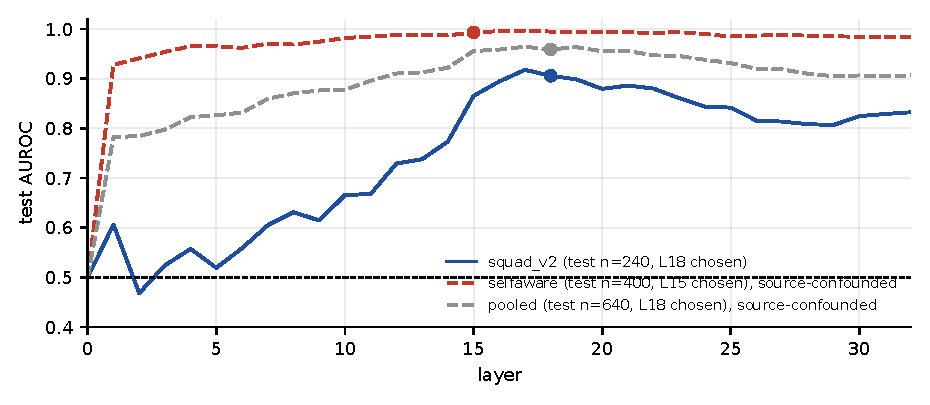
\includegraphics[width=0.85\linewidth]{figures/fig_layers_all.pdf}
\caption{Test AUROC by layer for the logistic probe on each dataset. Dashed curves are source-confounded (SelfAware, pooled). Dots mark the layer chosen on validation.}
\label{fig:layersall}
\end{figure}

\begin{figure}[t]
\centering
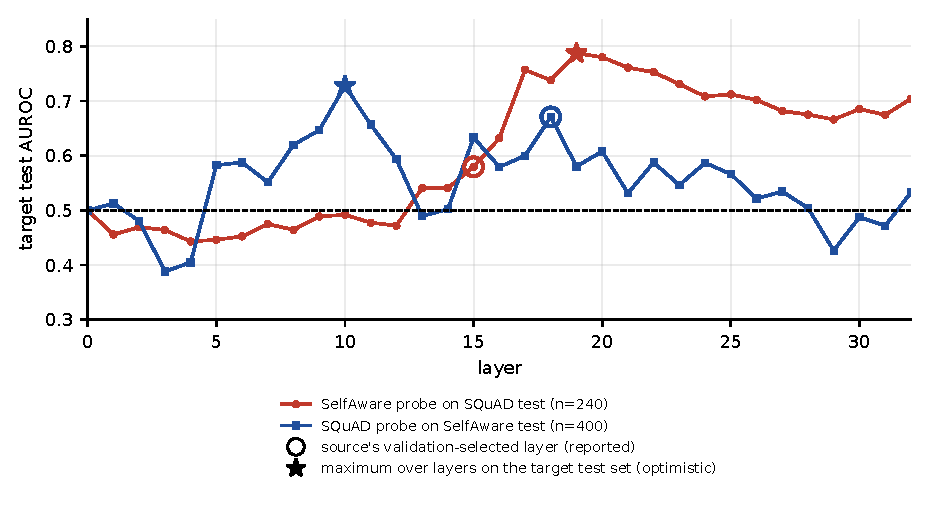
\includegraphics[width=0.85\linewidth]{figures/fig_transfer.pdf}
\caption{Cross-dataset transfer by layer. Circles mark the source dataset's validation-selected layer, which is the reported figure; stars mark the maximum over layers on the target test split, which is chosen on the target test set and is optimistic.}
\label{fig:transfer}
\end{figure}

\begin{figure}[t]
\centering
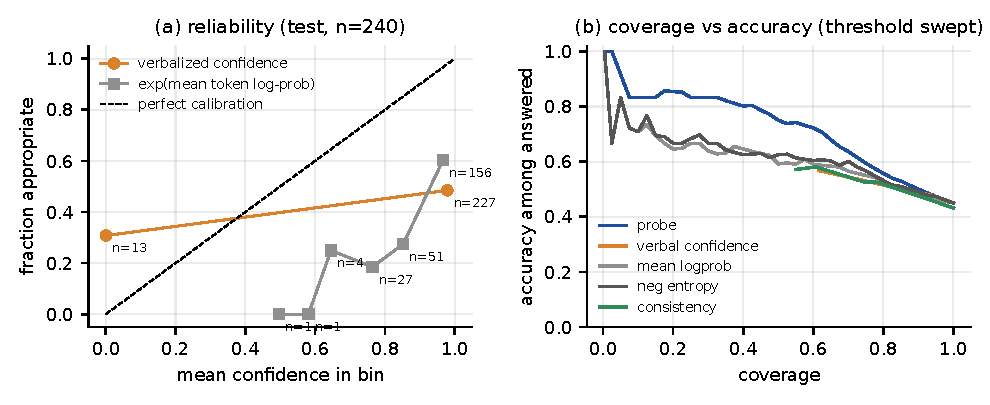
\includegraphics[width=0.95\linewidth]{figures/fig_reliability_coverage.pdf}
\caption{(a) Reliability of verbalized confidence and of the exponentiated mean token log-probability on the SQuAD test split; ``fraction appropriate'' counts a correct answer or an abstention on an unanswerable item. (b) Accuracy among answered items as coverage varies, for each signal's own threshold sweep (not tuned). The consistency curve uses the 51 items that have a score. Items answered on an unanswerable question count as wrong, so the ungated accuracy is 0.45.}
\label{fig:rel}
\end{figure}

\begin{figure}[t]
\centering
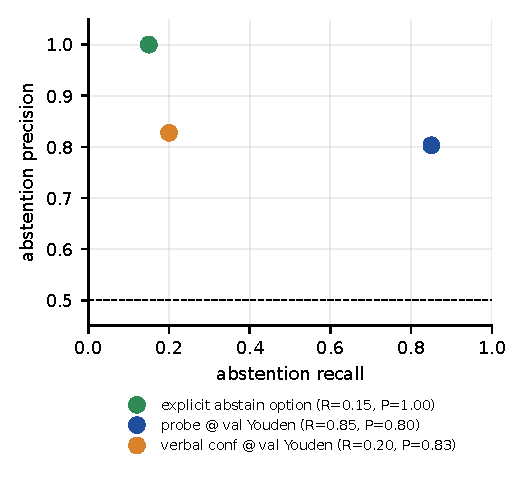
\includegraphics[width=0.52\linewidth]{figures/fig_operating_points.pdf}
\caption{Precision and recall for flagging unanswerable SQuAD test items: explicit abstain option, probe at its validation Youden threshold, and verbal confidence at its validation threshold (n=240).}
\label{fig:ops}
\end{figure}

\begin{figure}[t]
\centering
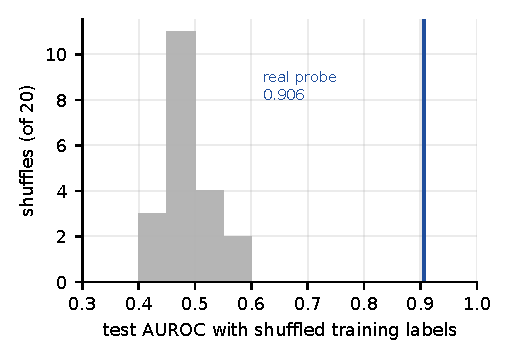
\includegraphics[width=0.5\linewidth]{figures/fig_shuffle.pdf}
\caption{Distribution of test AUROC over 20 shuffled-label runs on SQuAD 2.0, with the real probe's value marked.}
\label{fig:shuffle}
\end{figure}

\section{Reproducibility details}
The run used \code{torch} 2.11.0 (CUDA 12.8 build), \code{transformers} 5.22.2, \code{bitsandbytes} 0.50.2, \code{numpy} 2.5.4 and \code{scikit-learn} 1.9.1, with seed 13. The full run took 4,403 seconds for 3,200 items. Hidden states were stored in half precision and analysed in double precision. Configuration: 600 questions per class from SQuAD 2.0 dev, 1,000 per class from SelfAware, 60/20/20 splits, probe $C=1$ with at most 1,000 iterations, ten ECE bins, confidence cut 0.8, 300 bootstrap resamples, 20 label shuffles, consistency with five samples at temperature 0.7 on a hash-selected 25\% subset. The scripts that regenerate every figure and table in this report from the run's JSON files are in the \code{writeup/scripts} folder of the repository.

\end{document}
